\chapter{需求对话识别数据集构建与模型实现}

本章主要介绍从数据集爬取、数据预处理、数据标注、数据集构建到代码工程实现等部分,对{\tool}的工作流程结构进行阐述,并且介绍{\tool}在工业生产环境部署流程情况。
\section{数据爬取}
我们的数据是通过Scrapy \footnote{https://scrapy.org/}爬取的。Scrapy是用Python实现的一个为了爬取网站数据、提取结构性数据而编写的应用框架。Scrapy常应用在包括数据挖掘,信息处理或存储历史数据等一系列的程序中。通常我们可以很简单的通过Scrapy框架实现一个爬虫,抓取指定网站的内容或图片。如图\ref{fig:scrapy}所示,Scrapy主要有以下组件构成:Scrapy Engine,Scheduler,Downloader,Spiders,Item Pipeline,Downloader middlewares,Spider middlewares。
\begin{figure}[htbp]
    \centering
    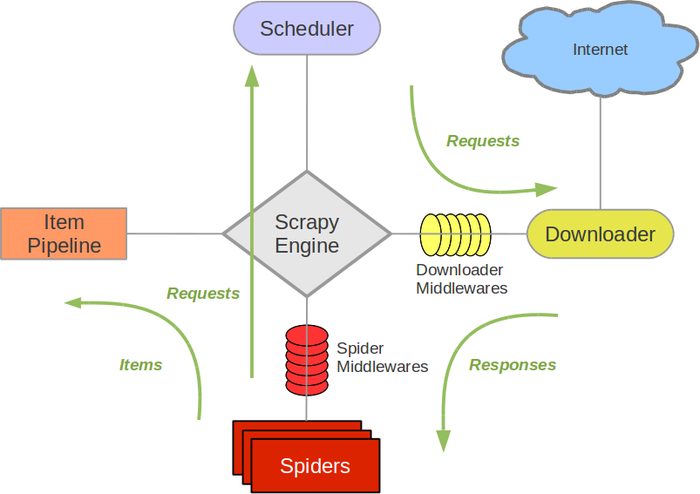
\includegraphics[width=0.6\textwidth]{Img/scrapy.png}
    \bicaption{Scrapy架构图}{The architecture of Scrapy}
    \label{fig:scrapy}
\end{figure}
Scrapy中需要用户自定义的一个核心的组件为Item,其存储了待爬取的对象结构信息。图\ref{fig:echelog}所示为AngularJS项目的IRC记录的格式与内容。
\begin{figure}[htbp]
    \centering
    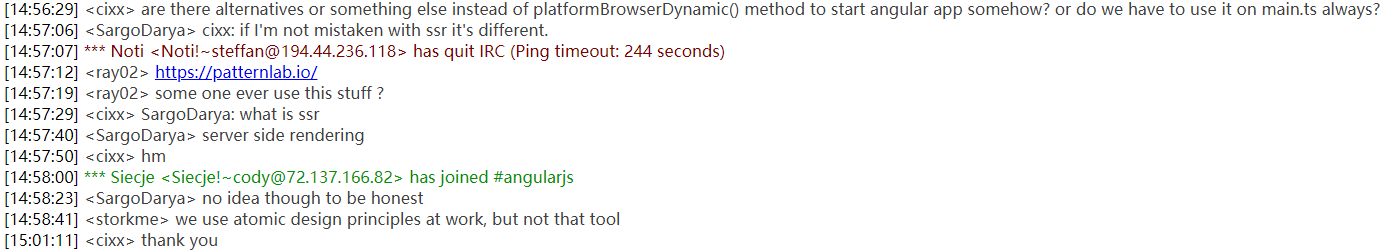
\includegraphics[width=\textwidth]{Img/echelog.png}
    \bicaption{AngularJS项目IRC记录样例。}{An example of AngularJS IRC channel.}
    \label{fig:echelog}
\end{figure}
因此针对IRC数据,我们爬取的Item对象的主要结构信息有:Timestamp,UserName和Message。
爬取的对象主要三个开源项目:AngularJS \footnote{https://angularjs.org/},Bootstrap  \footnote{https://getbootstrap.com/}和 Chromium \footnote{https://www.chromium.org/}. 我们选取这三个项目主要有以下几个原因:首先,它们是最近非常活跃的项目;另外这些项目中存在着较大的开源社区;这些项目中的开发者也非常活跃地使用在线聊天进行分享观点、有趣的见解以及讨论哪些特征需要在以后进行实现。例如,在过去的三年里,AngularJS社区里每周平均有2,823条对话。另外,这些历史对话在IRC Archive网站\footnote{https://echelog.com/}中进行存档并允许开放访问,其为我们的工作提供了丰富的语料资源。

\section{对话预处理}
我们首先对爬取到的文本中的非ASCII字符如emojis等转换成ASCII字符串。由于一些低频的Tokens,如URL、邮件地址、代码片段、HTML标签、版本号等对最后的分类结果不会产生帮助,因此我们对其分别使用\textit{<URL>,<EMAIL>,<HTML>,<CODE>,<ID>}等特殊Tokens进行替换。然后,我们使用Spacy \footnote{https://spacy.io/},一个优秀的包含分词、词性标注、词干还原等NLP处理功能的工具把句子进行分句、分词。为了减少词语形态学的影响,我们使用Spacy对单词进行词干还原和小写转换。

对对话数据进行基本的预处理之后,我们使用JK Kummerfeld等人\cite{kummerfeld2018large}发布的使用其标注数据上训练的模型对我们爬取的数据进行对话解耦,在经过人工审核之后,解耦之后的对话质量、可读性以及解耦的准确性较高,达到了可用标准。
对对话进行解耦之后,我们获取了大量的聊天对话。为了接下来进行数据标注的可行性,并且保证整个对话数据集的整体分布,我们从这三个项目中分别随机采样了400个对话。然后,我们从中过滤掉以下一些质量较低的对话:
\begin{enumerate}
    \item 使用非英语文本的对话
    \item 包含大量代码和Stack Traces信息的对话
    \item 存在大量拼写错误和语法错误的低质量对话
    \item 包含Channel Robots的对话。
\end{enumerate}

\section{数据标注}
标注的对话可以用作我们评估效果的数据集。为了保证标注结果的正确性,我们建立了一个标注小组,由两名资深研究人员和四名博士生组成。他们都具有较高的英语水平,并且在软件开发方面做过深入的研究工作,或者为开源项目做出了积极的贡献。我们将团队分为两组。每个小组由一名负责人(高级研究员)和两名成员组成。每个负责人培训了相应成员如何标注标签并为成员提供咨询。成员对标签的标注结果由负责人进行审查,而每组负责人的结果由其他负责人进行审查。仅当对话在各小组之间的标注达成完全一致时,我们才接受此对话并将对话以及其标签加入到我们的数据集中。而当对话被标注为不同的标记结果时,我们将与所有六个人进行讨论,然后通过投票决定最终标签。表\ref{tab:dataset}为爬取到的所有数据集和我们标注的数据集的统计情况。我们总共从三个开源项目中收集了65,428个对话,并花了720人/小时的时间来标注1,035个对话(总体数据集的1.6%)。

\begin{table}[htbp]
\bicaption{标注对话的统计详情}{The statistic of labeled dialogues}
    \label{tab:dataset}
    \centering
    \footnotesize% fontsize
    \setlength{\tabcolsep}{4pt}% column separation
    \renewcommand{\arraystretch}{1.2}%row space 
\begin{tabular}{|c|c|c|c|c|c|c|}
\hline
\multirow{}{}{} & \multicolumn{3}{c|}{全部聊天记录数据}    & \multicolumn{3}{c|}{抽取样本} \\ \cline{2-7} 
                  & 时间区间          & 对话数   & 句子数    & 对话数    & 句子数     & 特征请求数  \\ \hline
AngularJS         & 2016.5-2019.4 & 38266 & 406553 & 316    & 9220    & 36     \\ \hline
Bootstrap         & 2014.7-2019.5 & 10358 & 58871  & 379    & 2371    & 76     \\ \hline
Chromium          & 2015.5-2019.7 & 16804 & 118890 & 340    & 4465    & 27     \\ \hline
\multicolumn{2}{|c|}{总计}          & 65428 & 584314 & 1035   & 16056   & 139    \\ \hline
\end{tabular}
\end{table}
\section{孪生网络数据集构建}

不同于传统的文本分类模型,我们在数据集构建阶段需要分别对训练集和测试集进行Pair-Instance数据集构建。因此,我们针对p-FRMiner和FRMiner同时实现Single-Instance和Pair-Instance的数据集构建方法。对于p-FRMiner和FRMiner,我们同时实现两种数据集读取方式:lazy读取和一次性加载内存方式。其中lazy方式每次读取一行,然后构建对应Instance,也可以每次读取并构建一个Batch的Instance,以避免数据集过大不能同时加载到内存从而导致的程序运行问题。

对于数据集构建和接下来模型实现方面,我们使用AllenNLP\footnote{https://allennlp.org/},一个基于PyTorch\footnote{https://pytorch.org/}构建的开源NLP库。其中p-{\tool}和{\tool}实现的数据集读取类均继承AllenNLP的\textit{Dataset Reader}类。
p-FRMiner实现的Dataset Reader中的Instance包含三个元素:dialog矩阵,矩阵的每一行为一个句子分词后的词序列,句子组成的行序列对应句子在原对话中的序列;pos-tag矩阵,矩阵的每一行为一个句子分词后对应的pos-tag序列,句子组成的行序列对应句子在原对话中的序列,因此,pos-tag矩阵中的每个元素对应dialog矩阵每个元素词的pos-tag;label标签,分别以\textit{feature}和\textit{other}代表\textit{feature dialog}和\textit{non-feature dialog}。

而FRMiner为了组建Pair-Instance,其Dataset Reader的实现方式与p-FRMiner的Dataset Reader有所不同。在构建训练集时,遍历原始Single-Instance数据集,对于一个Dialog Instance—— $Dialog_1$,我们从训练集中同时采样一个正样本,也即label为\textit{feature}的$Dialog\_pos$和一个负样本$Dialog\_neg$,和$Dialog_1$组成两个Pair-Instance,即$<Dialog_1,Dialog\_pos>$和$<Dialog_1,Dialog\_neg>$,为了控制数据增强后数据集的大小以及避免增大随机采样带来的误差,我们对以上流程在整个数据集上及进行$iter\_num$次。对于Pair-Instance,其有以下元素组成:dialog1矩阵,矩阵的每一行为一个dialog中一个句子分词后的词序列,句子组成的行序列对应句子在原对话中的序列;pos-tag1矩阵,矩阵的每一行为一个dialog中一个句子分词后对应的pos-tag序列,句子组成的行序列对应句子在原对话中的序列,因此,pos-tag1矩阵中的每个元素对应dialog1矩阵每个元素词的pos-tag;dialog2和pos-tag2矩阵同理为另一个dialog的分词以及分词后对应的pos-tag矩阵;label标签,分别以\textit{feature}和\textit{non-feature}代表\textit{feature dialog}和\textit{non-feature dialog};label\_tags标签,其形式如\textit{feature@non-feature},代表Pair-Instance中的两个dialog原始标签分别为\textit{feature}和\textit{non-feature},保存原始标签的目的是为在训练集和测试集上进行类别推断而进行针对Single-Instance的效果评估。

在获取p-FRMiner和FRMiner对应的Instance后,我们需要讲Instance矩阵转为向量化表达从而进行训练。这里,我们使用AllenNLP的\textit{ListField}、\textit{TextField}和\textit{LabelField}将原矩阵的字符串元素如词、pos-tag、字符串label转为对应索引。然后AlleNLP在以上类里面将原始矩阵转换为以索引表示的神经网络输入数据集。

\section{分层上下文敏感对话模型构建}



模型构建部分我们主要继承AllenNLP的\textit{Model}方法,其实现了NLP中一些常见的方法,如Vocabulary中word到index的映射、参数初始化、正则项等。对于分层的上下文敏感对话模型实现部分按照如图\ref{fig:model}所示。考虑到NLP中批处理训练需要对不同长度文本句子进行padding,并且我们的输入不同于以[batch\_size, max\_sentence\_length]为输入的句子文本分类模型,其中max\_sentence\_length为大小为bath\_size的句子中的最长长度,对话模型的输入为[batch\_size, max\_utterance, max\_sentence\_length],其中max\_utterance为大小为batch\_size的输入对话中最大的句子数,max\_sentence\_length为所有对话中最长的句子长度,因此我们需要实现三维的padding方法,使对话输入Tensor能够进行批处理训练。不同于基本的TextCNN对句子分类的输入,我们在句子Embedding层使用不同大小卷积核的TextCNN,因此对于长度小于卷积核大小的句子,我们需要将其padding为卷积核大小长度。同样的,我们需要对pos-tag embedding 的三维Tensor进行padding,然后对word embedding和pos-tag embedding进行拼接。在对三维的输入Tensor进行padding之后,我们使用AllenNLP中的\textit{CnnEncoder}对batch中每个对话的每个句子使用TextCNN进行表示,由于对于TextCNN的输入为二维Tesnor,对此,我们将输入Tensor转换为形状为[batch\_size * max\_utterance, max\_sentence\_length]的二维形式。在经过TextCNN后,我们获取所有句子的embedding表示,然后还原为[batch\_size, max\_utterance, cnn\_out\_dimension],其中cnn\_out\_dimension为TextCNN的输出维度。在对话建模层,我们使用BiLSTM,以每个句子的embedding作为输入Term对对话句子的序列信息进行双向编码,然后,可以得到对话的最终向量化表示。为了在实验部分对p-FRMiner和FRMiner进行对比,我们对上下文敏感对话模型构建了线性分类层,并使用cross-entropy作为损失函数对Single-Instance进行分类,具体结构在实验部分介绍。

\section{孪生网络对话分类模型构建}
不同于传统的单文本目标分类任务,孪生网络使用两个相同结构、共享参数的编码器对文本进行embedding,然后使用相似度度量层对Pair-Instance进行相似性评估。我们对此并没有在代码中实现两个相同的网络,而是将两个对话分别输入到4.5中的一个上下文敏感对话模型中得到两个对话的embedding表示。针对对话的相似度度量,我们构建双层、以Sigmod为激活函数的线性层作为黑盒网络,同时接受两个对话embedding拼接的结果作为输入,输出为对话的相似性概率。因为我们在Pair-Instance数据集构建的过程中构建了相似度标签-\textit{same}和\textit{diff},因此相似度度量网络在输入对话和对应的label下可以进行训练并更新参数,从而拟合领域特定的对话相似性度量函数。对于label为\textit{same}和\textit{diff}的Pair-Instance数据,在经过以上下文敏感模型为基模型的孪生网络和相似度度量层之后,其输出分类为\textit{same}和\textit{diff}的概率值,其为一个二分类问题,这里,我们使用cross-entropy作为损失函数对模型参数进行更新优化。


\section{训练及模型调参}
我们对于训练过程使用AllenNLP的\textit{Trainer}类,其实现了一些神经网络训练过程中常用的方法,如序列化保存、GPU训练、数据集加载、梯度裁剪、TensorBoard可视化等。训练过程中所需要的参数保存在json文件中,AllenNLP加载json文件并初始化\textit{Trainer}类,然后开始进行训练以及评估测试。

对于超参数,我们使用Grid Search\cite{Bergstra2012Random}作为参数选择方法以获得最佳效果。pos-tag向量的维度为50,与单词向量相同。然后,我们可以使用$s=[w_1,w_2\dots w_n]$ 作为句子的表示形式,其中$w_i=[we_i\oplus pos_i]$。为了获得由不同尺度的局部信息组合而成的更充分的语义信息,我们对句子应用具有不同大小的多个卷积核。我们设置了4种不同的卷积核大小,分别是2、3、4、5,每类卷积核有25个。BiLSTM的输出尺寸为300(每个方向150)。我们使用线性层作为相似性度量层,然后将300维向量映射到两个值,这些值表示两个类别的概率得分。由于该任务可以视为分类问题,因此我们将交叉熵用作损失函数。

此外,为避免过拟合问题,我们以0.1的dropout rate对输入向量进行Dropout \cite{srivastava2014dropout},这意味着将随机屏蔽10%的神经元以减少每次批量训练中需要训练的参数。我们还使用了Early Stopping\cite{prechelt1998early}的策略,如果测试数据集的效果在10个Epoch内未提升,则训练过程将停止。对于神经网络的优化器,由于Adam\cite{kingma2014adam}对梯度的一阶矩估计和二阶矩估计进行综合考虑,并且其具有自适应性能好、参数的更新不受梯度的伸缩变换影响等特点,我们使用Adam优化器对模型参数进行更新优化。

\section{实际工作流应用场景部署}
我们的方法可以通过将{\tool}集成到发布团队的工作流中帮助收集群体需求。首先,发布团队需要构建聊天信息监测器或者爬虫来定期从公司的聊天平台收集对话文本信息。然后,使用自动化脚本\cite{kummerfeld2018large}来对原始对话文本进行预处理和对话解耦。接下来,通过前面介绍的对话表示和对话分类过程,{\tool}可以记录所有在表达特征请求的对话。而发布团队可以使用RSS(Really Simple Syndication)订阅定期监测收集到的隐含的特征请求对话结果。另外,由于开发者倾向于使用较为一致的方式在对话中表达特征请求,如“需要在下个版本中实现某功能”、“某功能将会一种解决方法/改进”等,因此仅当数据集的质量或聊天内容发生较大的偏移时{\tool}需要进行重新训练,否则{\tool}不需要经常进行重新训练。

% 另外,考虑到开发环境中尤其是开源社区会存在多种语言的对话如英文等,我们的方法也能很好的集成到其他语言环境中。 In addition, {\tool} can be applied to the other languages since our deep contextual dialog model has a strong ability in capturing semantic patterns. When switching to other languages, {\tool} users need to adapt the pre-trained word embedding model to the specific language. They also need to consider to apply extra preprocessing according to the specific language, e.g., apply word segmentation to Chinese corpus. Another limitation of {\tool} on language switching is related to the pre-trained dialogues disentanglement model. A new dataset needs to be annotated for retraining the model, which may involve a relatively high cost.


\section{本章小结}

本章设计并实现了我们提出的{\tool},并针对数据集构建过程进行介绍。首先我们介绍数据爬取、对话文本预处理、通过构建标注团队进行数据标注以及Pair-Instance数据集构建。接下来从工程实现角度介绍分层上下文敏感对话模型构建、孪生网络对话分类模型构建以及训练阶段和调参阶段细节。最后我们介绍了{\tool}如何在工业实际场景进行部署。